\begin{problem}[04]
从物理上分析摆锤质量与单摆周期无关的原因.
\end{problem}
% --------------------------------------------------------------------
\begin{solution}
\begin{minipage}[c]{0.8\linewidth}
\begin{itemize}
\item \textbf{证明}: 对于如右图所示的单摆, 摆长为$l$, 选取自然坐标系, 摆锤的的位置可由弧长$s=l\theta$确定, 摆锤受到的合力沿垂直于摆长的方向, 大小为$f = mg\sin\theta$, 因此摆锤加速度$a$为
\[
a = \frac{f}{m} = g\sin\theta = \frac{d^2s}{dt^2} = l\frac{d^2\theta}{dt^2}
\quad \Longrightarrow \quad \ddot{\theta} -\frac{g}{l}\sin\theta = 0
\]
显然上式最终得到的运动学方程中不含摆锤质量, 可见摆锤质量与单摆周期无关.
\end{itemize}
\end{minipage}
\begin{minipage}[c]{0.2\linewidth}
\begin{center}
\usetikzlibrary{%
    decorations.pathreplacing,%
    decorations.pathmorphing,arrows
}
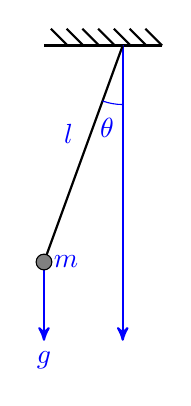
\begin{tikzpicture}[ media/.style={font={\footnotesize\sffamily}},
    wave/.style={
        decorate,decoration={snake,post length=1.4mm,amplitude=2mm,
        segment length=2mm},thick},
    interface/.style={
        postaction={draw,decorate,decoration={border,angle=-45,
                    amplitude=0.3cm,segment length=2mm}}}]
\draw[thick,interface] (0.5,3.75)--(-1,3.75);
\draw[->,>=stealth',thick,blue](0,3.75)--(0,0);

\draw [thick](0,3.75)--(-1,1) node[midway,above left,blue]{$l$};
\draw [blue,->,>=stealth',thick] (-1,1) -- (-1, 0) node [below]{$g$};
\draw [fill=gray](-1,1) circle(0.1) node [right,blue]{$m$};
\draw[blue] (0,3) arc(-90:-110:0.75);
 \node[blue] at (-0.2,2.7) {$\theta$};
\end{tikzpicture}
\end{center}
\end{minipage}
\begin{itemize}
\item \textbf{分析}: 摆锤的运动完全由重力加速度决定, 摆锤的运动是一个纯运动学的问题, 与质量无关, 所以摆锤质量与单摆周期无关, 因此\textbf{上述证明可以直接不引入质量}.
\end{itemize}
\end{solution}
